\documentclass{article}
\usepackage{fontspec}
\usepackage{parskip}
\usepackage{graphicx}
\usepackage[backend = biber, citestyle=numeric]{biblatex}
\addbibresource{plan2.bib}

\setmainfont{Noto Sans}

\begin{document}
\title{\textbf{Plan and Schedue for 2021 - v2}}
\author{James Engleback}
\maketitle
\tableofcontents

\section{Overview}
\subsection{Aim and context}
This project has two peices of work both with the aim to engineer a P450 BM3 mutant with some sort of metabolic activity towards an important herbicide for use in herbicide-resistant crops. % broad aims
\par
Herbicide resistant crops can be engineered by introduction of a P450 that can hydroxylate the target herbicide, priming conjugation with glutathione via Glutathione-S-Transferases (GSTs) and sequestration into the vacuole.
\par
Given the promiscuity of GSTs, there may be flexibility in the hydroxylation site of the herbicide. Therefore, the specific aim of this project is to engineer candidate P450s to hydroxylate a herbicide at any postion for further testing in plants by Syngenta. % end point
\par
Candidate P450s can be transformed into a model crop (e.g. tobacco) and evaluated for efficacy in glasshouse-based herbicide challenge trials.  % spray test
\par
\subsection{P450 Engineering Approaches}
Two approaches are being taken to engineer and then test variants of P450 BM3 with activity towards mesotrione - an important herbicide. Each approach will be written into a thesis chapter. % scope
\par
One approach uses a combination of classical structure prediction and molecular docking methods as a simulation envorinment for virtual directed evolution driven by a genetic algorithm. % broad on enz
\par
The other uses a deep learning model built to predict binding ($pK_d$) for a given enzyme sequence and ligand SMILES. Model predictions of $pK_a$ towrads mesotrione can be used as a fitness criteria in virtual directed evolution experiments at a large scale.% broad on rio
\par
Both approaches will generate pools of candidate mutants that will need to be tested for efficacy in the lab. Candidate mutants will be expressed, purified and evaluated for: $K_d$, $K_m$ and $K_{cat}$ towards mesotrione, and have product formation confirmed via LCMS. % both  lab valdation

\section{Structure-Based Design}
\subsection{Overview}
This aproach uses classical protein structure prediction methods and molecular docking to simulate herbicide binding in the acive site. The simulation is used to create a virtual directed evolution experiment where a genetic algorithm uses a heuristic fitness estimate to generate candidate pools of mutants with predicted herbicide binding.  % overview
\par
\subsection{Related Work} % related work
In the source material for template-based structure prediction and molecular docking \textcite{rosettadock} predict the structure of lysozyme mutants based on a crystal template structure using side chain repacking and loop remodelling. They then compare the accuracy of \textit{rosetta} and \textit{autodock vina} docking performance based on a ligand bound reference crystal structure. They find that the structure prediction methods used are sutable for predicting the structure of near mutants and that \textit{rosetta} docking methods perform better than \textit{autodock vina} but incurs a significant computational cost. \textit{autodock vina} still performed reasonably well.  % rosetta paper todo - refs, reword, performance metrics.

\subsection{\textit{enz}} % enz
The simulation environment is contained in a python package built for this project, \textit{enz}. The scope of \textit{enz} is template-based structure prediction using \textit{pyrosetta} and molecular docking using \textit{autodock-vina} as backends. % enz
\par
Currently, \textit{enz} only uses side-chain repacking for structure prediction and rigid side-chain molecular docking using \textit{autodock vina}. \textit{enz} works robustly and is extensible to new and modified docking and structure-prediction methods. % technical
\textit{enz} is ready to deploy in virtual directed evolution in its current state, but modifications that may significantly improve accuracy have been identified:% readiness
\begin{itemize} % proposed improvements
	\item \textbf{Flexible docking} - where \textit{vina} treats active site side chains as flexible. This is can be imlemented with \textit{vina}, and is a viable route of investigation. 
	\item \textbf{Flexible (loop) remodelling} - where \textit{pyrosetta} treats unstructured regions as loops and optimizes their conformation using Cyclic Coordinate Descent (CCD). \textit{pyrosetta} has an implementation of CCD which can be integrated into the \textit{enz} \texttt{refold} function.
\end{itemize}
\subsection{\textit{enz} Benchmark}
\textcite{rosettadock} benchmark template-based structure prediction and ligand docking using both \textit{rosetta} docking and \textit{autodock vina} against mutant lysozyme strucutres. % rosetta paper benchmark
% rosetta benchmark insights
\par
A performance benchmark will need to be established to evaluate efficacy of \textit{enz} and test experimental branches. The benchmark will be based on structure prediction and docking RMSD to reference ligand bound crystal structures of BM3, of which there are X. This can be generalized to other structures for which there also exists a structure of a close mutant in future. % validation
\par
Discrepencies between ligand conformations in BM3 crystal structures and molecular dynamics simulations exist and may suggest that the crystal structures represent one of several stable conformations. % bm3:md discrepancies
Therefore a suitable metric will have to be chosen carefully to reflect convential knowledge whilst avoiding bias towards \textit{enz}. At the same time it should be sensitive in the range that \textit{enz} improvements can affect. It would be very useful to plan a suitable metric with help from someone with domain knowledge in molecular dynamics, protein strucure and molecular docking - Sam, Linus and Nathan Kidley from Syngenta come to mind. % judgement -> metric, orientation and help

\subsection{Virtual Directed Evolution Overview}
Virtual directed evolution requires a sequence optimization algorithm and a sequence fitness function. In this case, a genetic algorithm is the sequence optimizer and mutant fitness is a score based on docking results of a target compound against the predicted structure. % overview
\par
The heuristic currently employed to estimate the desirability of each set of docking results is % heuristic
\begin{equation}
score = \frac{1}{n}\Sigma _{N} \Delta G_{i} \times d_{i}
\end{equation}
where $ \Delta G $ is free energy of the interaction calculated by \textit{autodock vina} (\textit{kcal / mol}) and $ d $ is the distance between the heme iron and the C5 of mesotrione for $ n $ in binding poses. Where C5 is the target carbon for hydroxylation. It may be sufficient for use in the genetic algorithm but can be flexibly changed if needed. % heuristic
\par
This effectively ammounts to an average distance between the target carbon and the catalytic iron weighted by binding energy. % heuristic
\par
The genetic algorithim employed as a sequence optimizer randomly mutates input sequences at a single position randomly chosen from a set of active site residues to generate a pool of mutants. Fitness of each is queried using \textit{enz} and the heuristic discussed above and the $n$ fittest mutants are randomly recombined with eachother and randomly mutated again to repopulate the pool. % ga
\par
Mutant fitness is evaluated in parralel, enabling scale up to hardware capacity. It can run on a small virtual private server (VPS) and run 20 iterations with a batch size of 20 mutants over 2 days, though generally a large batch size results in faster convergence to good solutions. % ga parralelism

\subsection{Status, Readiness and Going Forward}
An implementation of the described virtual directed evolution is ready to run in its current state. More accurate predictions enabled by changes to \textit{enz} will result in a better pool of engineered mutants. % readiness
Since there is only time to make and test one batch of mutants generated by this process in the lab, final modifications to \textit{enz} will be made before the process is used to generate mutants to be made and tested in the lab. % wait
\par
3-5 days of work are required to attempt to implement the proposed changes to \textit{enz} and set up the virtual directed evolution algorithm on a suitable peice of hardware. The small VPS can be used if necessary. % timeline - programming
\par
The described changes to \textit{enz} will finish and virtual directed evolution will proceed in March. Work to construct expression plasmids for the candidate mutants can start after this. % rough schedule
The candidate mutants will be subject to the same validation process as that used for those generated by machine earning. This process is detailed in \textbf{Mutant Validation}. % ln validation

\section{Machine learning-based Design}
\subsection{Overview}
This piece of work aims to use machine learning model predictions of binding ($pK_d$) between an amino acid sequence and a ligand as a fitness function in virtual directed evolution experiments. % overview
\par
The model will be trained on in-house screening data of BM3 mutants' binding $K_d$ with herbicides and herbicide-like compounds. A high throughput assay has been developed for this work and screening has begun. % screen
\par
Similar to candidate mutants genereated in the \textbf{Structure-based Design} section, candidate mutants with predicted binding towards mesotrione will be expressed, purified and assayed for $K_d$, $K_m$, $K_{cat}$ and product formation with mesotrione. % lab - val
\par

\subsection{Related Work}
% ml protein engineering
% ligand prediction

\subsection{Screening}
The screen employed here measures $K_{d}$ between BM3 variants and ligands by measuring response of the P450s' UV-Vis absorbance profile to increasing ligand concentrations. % scope and overview
\par
The screening assay is a 384 well plate analog of traditional cuvette-based titration. Eight concentrations per ligand is sufficient for a reasonably accurate $K_d$ estimation, accommodating 48 compounds per plate. One plate takes 5 minutes to read in a \textit{BMG FluoStar} plate reader, and another 10 minutes to transfer data to the dedicated computer which limits the screening rate to a maximum 4 plates per hour. % throughput
\par
Over 2 days 12 plates (576 compounds) can feasible be set up by hand and screened against purified BM3 mutants.   % setup
\par
During development, automation of compound dispensing using a \textit{Labcyte Echo} was more accurate and reliable than dispensing by hand. Access to a \textit{Labcyte Echo} in Patrick Cai's group has been arranged, so there is scope for automation of this step.  % echo

\subsubsection{Assay Technical Details}
The Assay takes place in clear 384 well plates and uses 30 µl of ~10 µM BM3 in each well. % plate and prot
Test compounds are added in DMSO so that the final DMSO concentration is 5 \% in each well, which controls the mild binding activity between BM3 and DMSO. % dmso 5%
Assay buffer is 100 mM KPi \textit{pH} 7 and 1 \% bovine serum albumin (BSA) to mitigate BM3 precipitation. % bsa
UV-Vis absorbance by the test compounds is corrected for in a control plate with only compounds in buffer. % controls
Currently, compounds are dispensed into plates using a multichannel pipette from a set of master plates that contain serial dilutions $\frac{1}{2}$ of each compound. % serial dilution
Measurement of UV-Vis absorbance between 200 and 800 nm is a capability of most \textit{BMG} platereaders, and is currently done on the Field group's \textit{BMG FluoStar} on the third floor. The total time to read the plate and store the data takes 15 minutes. % reading
\par
Setup of compounds can be done a day prior to the assay. Once BM3 is added to the plate, the assay remains stable at room temperature for at least an hour. % break points
\par
A minimum of 5 µl of compound stock (10 mM in DMSO) is used per plate plus an additional 5 µl for the control plate per batch. Therefore a batch of several mutants screened against a compound set at once is economical. % compound consumption
One plate of 48 compounds consumes 12 ml of 10 µM BM3 stock. BM3 purified from a 6 L expression will accommodate > 10 plates. % protein consumption
\par
Analysis is automated and generates a report for each test compound and assembles the $K_d$ calculations for each into a csv file for model training. % analysis
\textbf{Figure \ref{pilot_report}} shows an example report of a binding interaction between a BM3 mutant and a compound, generated in the recent pilot assay.

\begin{figure}
	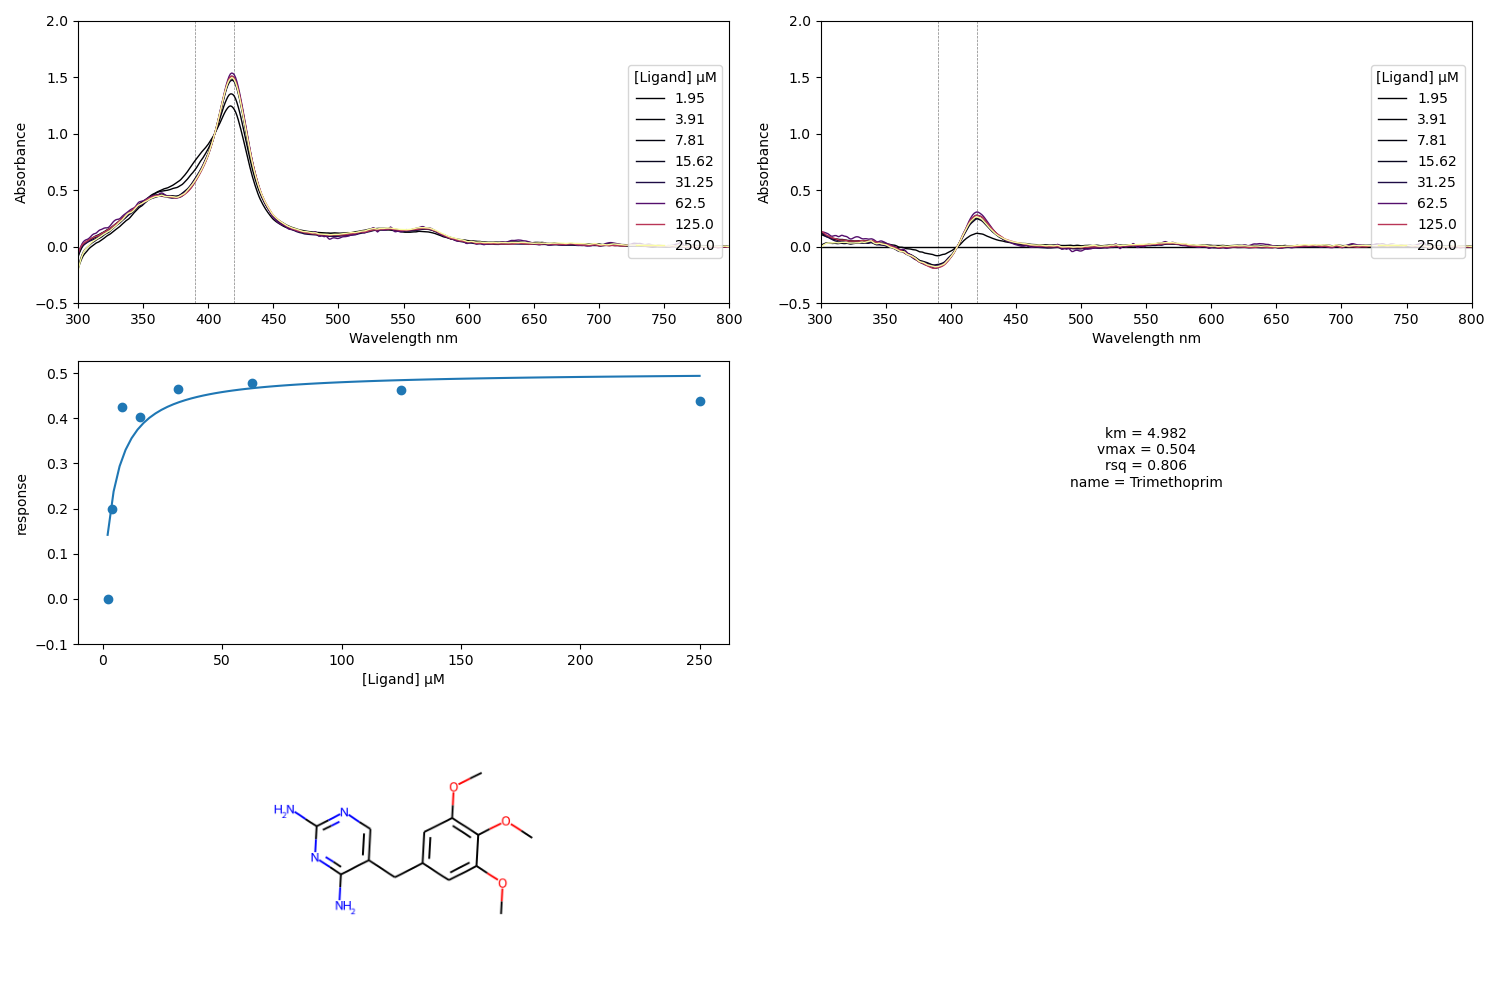
\includegraphics[width = \textwidth]{Trimethoprim.png}  % show report
	\caption{Example report from recent pilot assay showing response of BM3 mutants A82F to Trimethoprim \label{pilot_report}}
\end{figure}

% todo fignum and legend
\par
Currently anomalous experiments are easy to identify and discard manually however an effort is being made to automatically detect and remove anomalous data points rather than the all eight traces. % analysis

\subsubsection{Automating compound dispensing with the \textit{Labcyte Echo}}
During development, a \textit{Labcyte Echo} acoustic liquid handler was used to dispense compounds accurately and reliably. I gained extensive experience working with this machine  and can adapt the assay to use it fairly easily. Going forward, an effort to use the \textit{Echo} liquid handling robot again will be made, which greatly improves accuracy and reliability of compound dispensing - see \textbf{Figure \ref{echo_report}} for a report of a test using the \textit{Echo} to dispense lauric acid with BM3 wild-type. A notable difference in the data produced using the \textit{Echo} compared to that where compounds are dispensed by hand is the consistency of compound dispensing. In the figure the Michaelis-Menten curve has not fit correctly because it is anchored by its $Y$ intercept at 0, however this is easily handled.  % justify echo
\par
Because of the improvement in pipetting accuracy, I will attempt to re-establish the \textit{Echo} as part of the assay. This will also eliminate the risk of mis-dispensing compounds when pipetting, which is a very real risk. Additionally it increases scalability of the assay.
The Cai group's \textit{Echo} is relatively available compared to the FBRH's machine, so access should not be a problem. 
\par
Dispensing instructions for the \textit{Echo} were generated with a python script which will need to be re-written. I plan on packaging it as a more flexible tool that can be applied to other assays in future.
 
\begin{figure}
	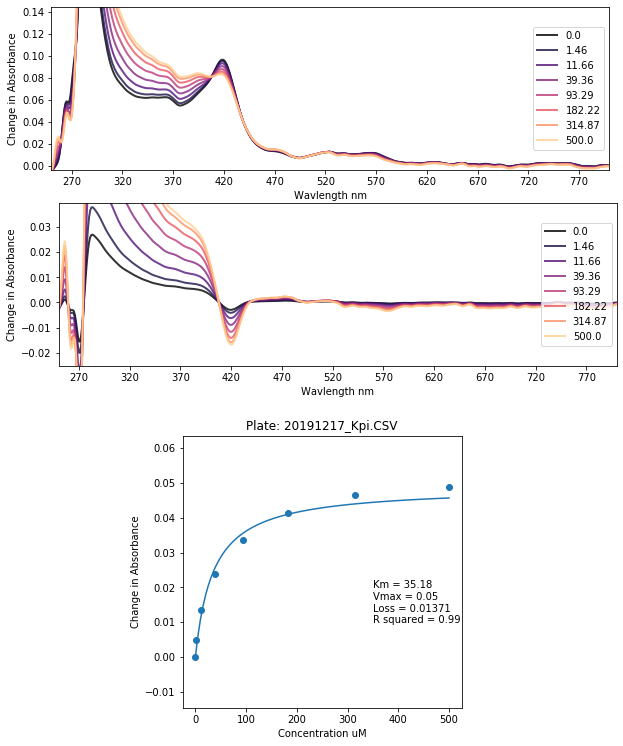
\includegraphics[width = \textwidth]{echo-report.png} 
	\caption{Report from an assay during development using the \textit{Echo} to dispense lauric acid into wells. \label{echo_report}}
\end{figure}

\par
I have been liaising with the person responsible for the \textit{Echo} in the Cai lab and can make an attempt next week to incorporate it into my pilot screening experiment. If successful, the screen will proceed with use of the \textit{Echo}. % format going forward
% timeline
\pagebreak

\subsubsection{Mutant Inventory and Purification}
I currently have the following mutants purified and ready to screen: % status and inventory
\begin{itemize}
	\item Wild type
	\item A82F
	\item A82F/F87V
	\item T268A 
	\item T268N 
\end{itemize}
I have cell pellets ready to purify for the following mutants:
\begin{itemize}
	\item K97C
	\item P393A - 118g
	\item K97C - 88g
	\item A264E - 77g
	\item A82F - 50g
	\item F393W - 67g
	\item F393A - 36 g
\end{itemize}
Additionallly, I currently have plasmid stocks for the following mutants:
\begin{itemize}
	\item A330P
	\item E267P
	\item F87A
\end{itemize}
\par
Mutant expression plasmids are created by site-directed mutagenesis from existing stocks. Success rate is reasonably good and a round of mutations can be introduced in a week with some luck. To mitigate the chances of a failed set of reactions, mutagenic PCR is done in batches.
\par
Expression is in BL21 (DE3) \textit{E. coli} cells grown in autoinduction TB broth. 3 hours of growth at 37°C followed by 24 hours of growth at 25°C is sufficient to yield 50-120 g of cell paste, which can yield 1 µmol of pure enzyme per 6 Litre expression - enough for 10 plates (480 compounds). % process
\par
Purification is one step nickel affinity chromatography and takes 2-3 days per mutant, however purifications can be batched. Based on prior batch purifications, maximum estimated purification capacity is 4 mutants in one week. % timeline
\par
6 BM3 mutants can be purified from existing cell pellets over the course of March, during which time communal autoclaves are due to be serviced. % queue march

\subsubsection{Compound Selection}
Compound library diversity is required to minimize bias of the model when trained. Herbicide-likeness may also improve the models' accuracy over the chemical space occupied by herbicides. % requirements
I have been using filtering rules based on \textit{ref} and the \textit{MaxMin} algorithm to pick $n$ diverse compounds. This method can select a diverse set f $n$ herbicide-like compounds from a given set. % method
\par
This compound selection method has been applied to an in-house compounds library of 979 FDA-approved compounds for a pilot screen. Since 48 compounds pass the herbicide-likeness filtering, it is feasible to proceed with screening with compounds we already have with 9 additional in-house herbicides. Note that the Library has been stored at -80°C for 4 years and there is some concern over compound degradation and contamination. % fda
\par
The same compound selection method can be applied to the database of compounds available via \textit{Molport}, a compound aggregator. Quotes (including lead time) of candidate screening libraries can be autogenerated using the \textit{Molport} API in order to find a suitably cheap set. Compounds can arrive within 4 weeks of ordering and handling can be covered by a single COSHH form. \textit{Molport} can deliver in many formats, including as 10 mM solutions in DMSO in a \textit{FluidX} plate, which is most convenient to me. % molport
\par
Going forward, a set of 96 compounds from the in-house FDA library and the panel of 9 herbicides will be screened until it is demonstrated that additional compounds are required. % going forward

\subsubsection{Pilot Screen - Initial Results}
A screening set was selected from the in-house FDA library using the method described and combined with 9 herbicides from in-house stocks including mesotrione for a total of 96 compounds. Of this set, 48 were screened against three BM3 variants due to a planning oversight that can be mitigated next time. % screening set
\par
Compounds were located in cold storage based on the manufacturer-specified positions, however they did not correspond to the serial numbers which were used to retrospectively identify each compound. This necessitates a second attempt at the pilot screen and a cataloging effort of the library, due to take place in the week starting 2 March. % mixup and redo
\par
Despite the mentioned issues the initial pilot assay was useful to develop an analysis package and gauge the resource requirements of the assay. As a result, it was decided that compound dispensing should happen the day before measurement to avoid the same time constraints encountered last time. % initial results
\par
Going forward, the pilot assay will be re-attempted in the first week of March with the following differences: % conclusions and going forward
\begin{itemize}
	\item Compounds will be dispensed into plates using the \textit{Echo}
	\item Compounds will be dispensed ahead of time to allow room for the \textit{entire} screening set to be tested against the 5 purified BM3 variants.
	\item The correct compounds will be screened
\end{itemize}
\par
Following this test, additional mutants will be purified and screened in March whilst additional mutants will be prepared. Screening will continue with the existing compounds until it is clear that purchasing of additional compounds is required.

\subsection{Additional Mutants for screening}
Additional expression plasmids can also be assembled in March. Work is ongoing to identify BM3 mutants with known altered substrate scope that can be obtained with few point mutations relative to existing stocks.  % pcrs march
% table of mutants
\par

The selection will be angled towards ring-containing substrates since most herbicides contain ring systems. The current goal is to ifentify 6 mutants for further screening. Literature is a rich source of mutants and 6 mutants with diverse substrate scope is faesible \textcite{wong}. % summarize
\par
\textbf{Table \ref{bm3_table}} contains a selection of promising mutants found in literature so far. The \textit{LVQ} and \textit{GVQ} mutants show relatively broad substrate scope and can be built in two steps from existing stocks.

\begin{table}
	\begin{center}
		\caption{Engineered BM3 Mutants\label{bm3_table}}
		\begin{tabular}{l|p{3cm}|l}
		\textbf{Mutant} & \textbf{Substrate scope} & \textbf{Pic} \\
		\hline 
		F87A/I263A/(A328I) & Nootkatone & 
\includegraphics[width = 2cm, height= 2cm, keepaspectratio=true]{nookatone.png} \\
		A328F & Limonene & 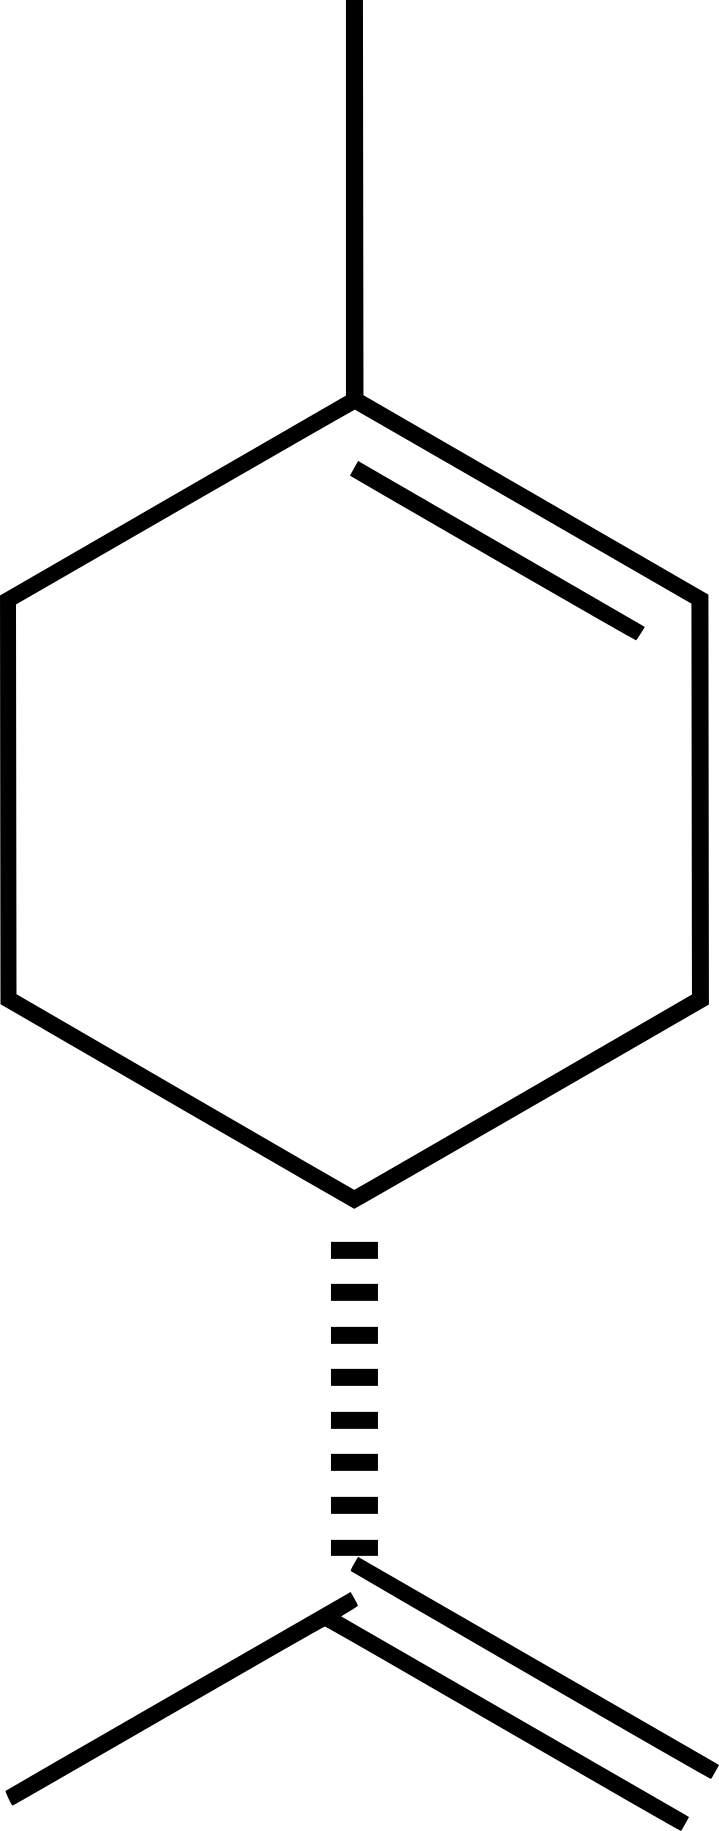
\includegraphics[width=2cm, height= 2cm, keepaspectratio=true]{limonene.png} \\
		R47L/Y51F & Alkylbenzenes (no heteroatoms) & 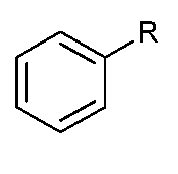
\includegraphics[width=2cm, height= 2cm, keepaspectratio=true]{alkyl-benzene.png} \\
			R47L/F87V/L188Q (LVQ) & Coumarins & 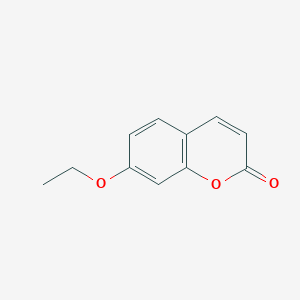
\includegraphics[width=2cm, height= 2cm, keepaspectratio=true]{7ethxycoumarin.png} \\ % this pic sucks
			A74G/F87V/L188Q (GVQ) & Indole, Lovastatinn, beta-ionine, organophosphates, polyaromatic hydrocarbons, chlorinated dioxins & 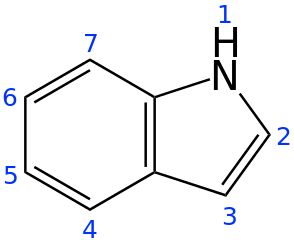
\includegraphics[width=2cm, height= 2cm, keepaspectratio=true]{indole.png} \\
	\end{tabular}
	\end{center}
\end{table}

%%% todo - which mutants and why - connecting the dots
\pagebreak

\subsection{Model} % model
The proposed model is combines two deep learning architectures that have proven efficacy in chemical data and sequence learning tasks. Graph neural networks are a class of model that are ideal for learning chemical data \textit{todo: ref} whilst transformers are very effective on sequence learning tasks. % architecture justification
\par
A model that combines transformers and graph neural networks has been constructed to estimate $pK_d$ between a given enzyme sequence and ligand SMILES and an overview is in \textbf{Figure \ref{rio}}. % architecture pic
\subsubsection{Architecture}
The model constructs a chemical graph from a smiles string, which is processed by a graph convolutional network and downsampled to a fixed-size embedding vector using set2set. Meanwhile the amino acid sequence string is downsampled using three 1D-convolutional layers and processed to a short, variable-length tensor which is downsampled into a fixed-size vector using the final hidden-state from an LSTM layer. % detail
The learned embedding vectors of the sequence and conatenated into a combined representation vector. A two layer perceptron provides a point estimate of binding likelihood. A diagram of the structure of the model is in \textbf{Figure \ref{rio}} % more detail
\par
\begin{figure}
	\caption{Graph illustrating the layers of the predictive model used in this work with layer types indicated.\label{rio}}
		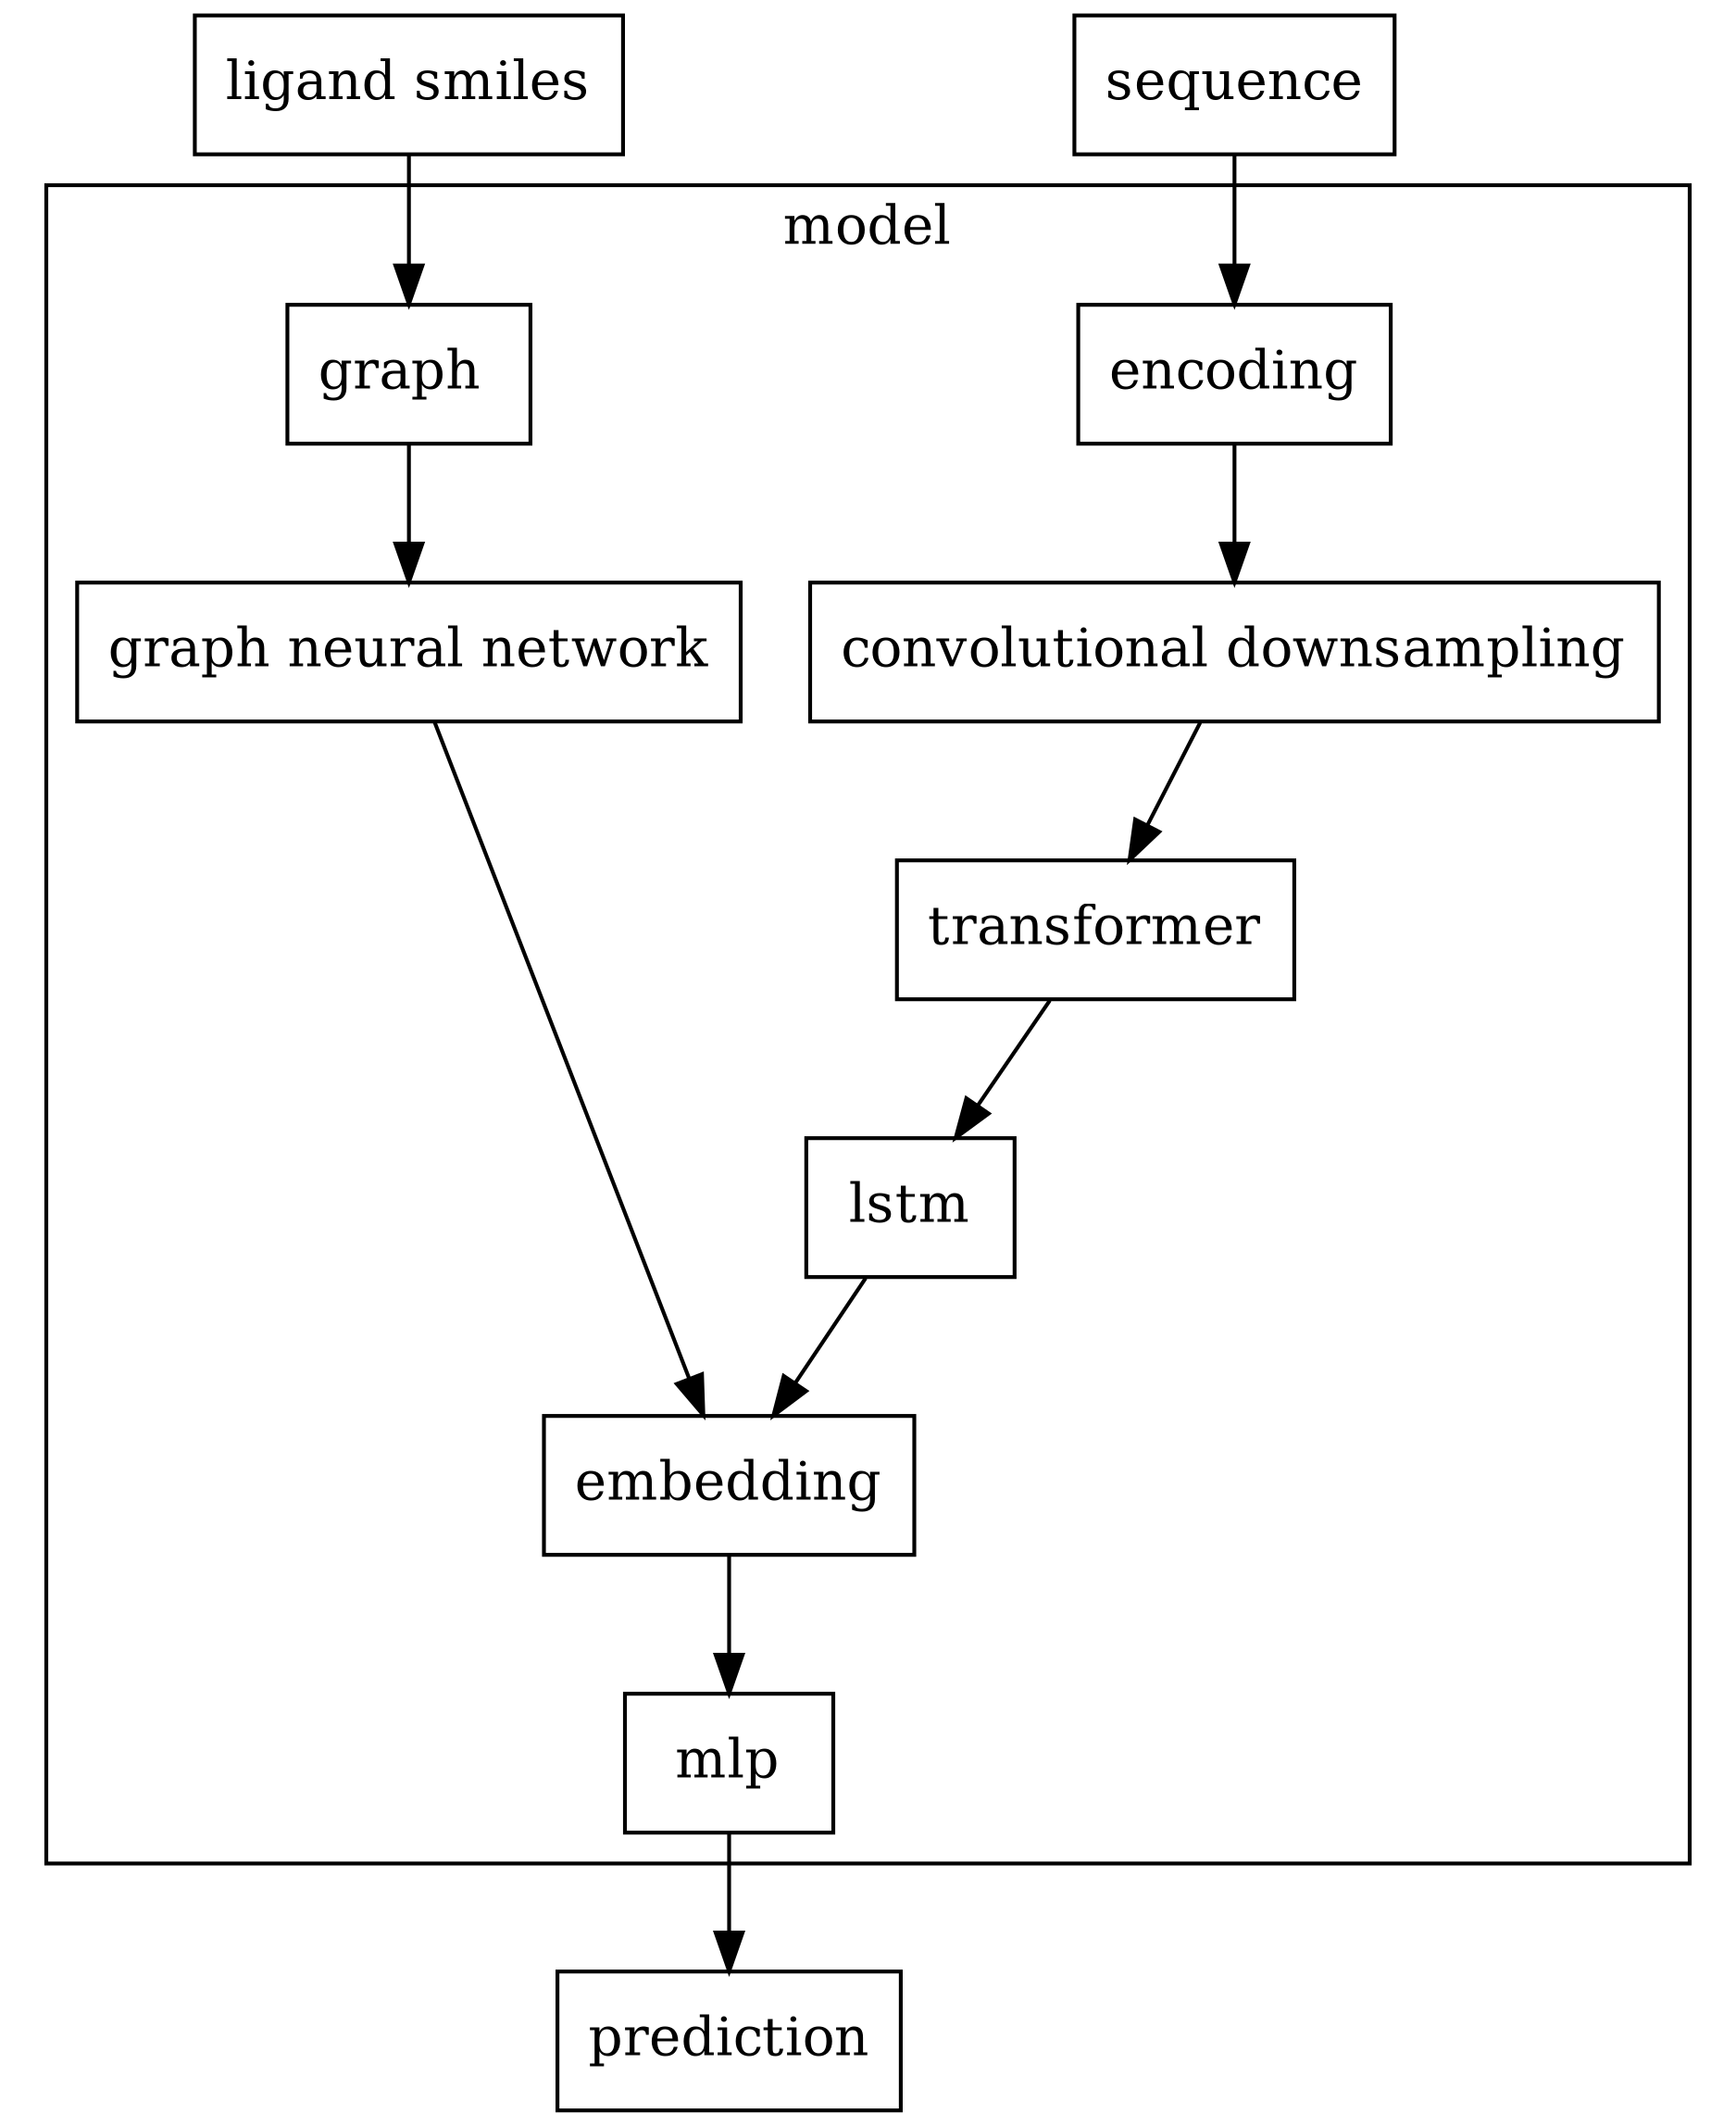
\includegraphics[width = \textwidth]{rio.png} \\
\end{figure}
\par
\par
\subsubsection{Transfer Learning}
Transfer learning is a popular approach to enhancing model accuracy and involves pretraining the model on a large, general dataset before transferring to a new task. The effect is a reduction in the number of samples required to train the model. Pre-training datasets do no necessarily need to be closely related to the target task, for example: models initially trained on the CIFAR 100 dataset (contains cars, animals etc. has been successfully re-tasked on phenotype identification from microscopy images. Transfer learning is predicted to drive commercial success \textit{Andrew Ng NIPS 2016 talk}. % xfer learning justification
%%% todo ref and clean
\par
The pre-training dataset has been mined from KEGG and currently holds roughly 0.2 million data points of enzyme sequence and smiles for reactants and products. I've identified changes to the data miner that could increase the dataset size close to $10^6$.  % kegg xfer data set
\par
The dataset contains only positive examples of probable enzyme-substrate pairs which necessitates generative-adversarial training, a common machine learning technique. % AN training
\par
\subsubsection{Generative-Adversarial Networks (GANs)}
In generative-adversarial training loops, the model competes with a generative-adversarial network (GAN) to discriminate between real data points and those generated by the GAN. Competitive training results in a GAN that generates realistic samples from a similar distribution to the training data whilst the predictive model predicts the likelihood of a given sample in the training distribution. This approach is utilised for sample generators (e.g. deepfake) and predictive models that have learned a data distribution (e.g. for anomaly detection). % GAN training overveiw todo - delete examples? 
\par
There is scope to monitor training by assessing the quality of the generated sequences and molecular graphs, indicating performance of the entire system. % monitoring pre training
Candidate models will be saved for later retraining on screening data. % save candidate models
\par
\subsubsection{Model-Based Mutant Design}
To design new mutants with predicted activity towards mesotrione (or any other herbicide) the model's predicted $pK_d$ between a candidate amino acid sequence and mesotrione is used as a fitness function. A genetic algorithm can be used to evolve a pool of new mutants for lab testing. % fitness 
\par
The model can evaluate a large number of binding predictions in parallel very quickly which enables a large scale virtual directed evolution experiment. In future work, alternative sequence search algorithms can replace the genetic algorithm for improved performance but genetic algorithms are the simplest case and should be sufficient for this use case. % ga  prediction speed
\par
Prediction uncertainty estimates are a result of \textit{ref dropout bayes} and can be used to inform decisions based on model predictions. % uncertainty estimates todo ref

\subsection{Status and Going Forward}
The pilot assay will transition into the screen proper in the first week of March using 9 herbicides including mesotrione and 48 herbicide-like compounds from the FDA library against 5 purified BM3 variants. An effort to use the \textit{Echo} will be made. % screening
\par
Pre-training and re-training will be attempted by the second week of March. A set of candidate models will be saved and training parameters will be swept. % pre-training
\par
Models will be evaluated on performance on the screening set. If no suitable model can be produced, a fall-back option is to investigate simpler models constrained to a select few amino acid positions. % evalutation
\par
The next 6 mutants for screening will be purified in March, batching 3 purifications to a lab week. Screening all 6 purified mutants will be batched to a week. % further screening
\par
Plasmid stocks of an extra set of mutants with known altered substrate scope will be designed and made in March. % extra mutants
\par
Expression and purification of these mutants may last from April-May. After these mutants are screened, then the project will transition into a mutant-generating and testing phase. 
\par
A pool of mutants will be engineered using a virtual directed evolution experiment using model predictions of binding activity towards mesotrione as a fitness function. 
\par
The pool of candidate mutants will be made in the lab and tested for $K_d$, $K_M$ and $K_{cat}$ and have an indication of product formation.

\section{Mutant Validation}
\begin{enumerate}
\item Expression and purification using nickel affinity chromatography
\item $K_d$ measurement with mesotrione using titration and UV-Vis spectroscopy
\item $K_{cat}$ measurement with mesotrione by monitoring reaction NADPH consumption by UV-Vis spectroscopy
\item Product analysis with LCMS where a hydroxylation at any position is considered a hit
\end{enumerate}

\section{Schedule}
\subsection{Feb - work done and work outstanding}
\subsubsection{Pilot Screen}
A pilot screen of 48 compounds against 3 BM3 mutants has been done. Lessons learned have helped inform the practicalities of the assay. I'm unsatisfied with the accuracy of dispensing compounds with a multichannel pipette so an \textbf{outstanding} task is to reimplement the \textit{Echo} as part of the assay. 
\subsubsection{Compound Selection}
48 compounds in the FDA Library are herbicide like, and will be used for screening alongside 9 real herbicides for now. The \textit{Molport} compound selection program needs some modifications to access the \textit{Molport} API to auto generate quotes and lead times, allowing me to choose the cheapest possible screening set.
\subsubsection{Improvements to \textit{enz}}
Still outstanding. Work done is refactoring the \textit{enz} \texttt{refold} function for extensibility to alternative folding methods. 3 Python Club sessions on \textit{enz} were taught.
\subsubsection{Virtual Directed Evolution with \textit{enz}}
Still outstanding. Work done is prepare a script that can run the experiment. 

\subsection{March}
\subsubsection{Spillover from Feb}
\begin{itemize}
	\item \textit{enz} improvements
	\item run virtual directed evolution
	\item finish pilot with \textit{Echo}
	\item set up lcms pipeline
\end{itemize}
\subsubsection{Structure-based}
In March I will prepare DNA stocks for mutants predicted using \textit{enz}. The maximum number of rounds of site-directed mutagenesis will be three, so this work can be fit into one month.  % lab - dna work
Any available slots for incubator and centrifuge time will be booked for next month. % prepare testing
I will create benchmarks for mesotrione product detection by LCMS using BM3 A82F/F87V I have on hand. This establishes a pipeline for upcoming product detection experiments. % lcms practice

\subsubsection{Machine learning-based}
I will proceed with screening the 48 herbicide-like compounds from the FDA-approved library and the 9 herbicides I have with the 5 purified mutants. I will also purify and screen the cell pellets I have (5 unscreened mutants) and screen them too.
I will decide on whether additional compounds should be acquired from molport and order if necessary. Lead time is 4 weeks so I will be able to screen these compounds with remaining mutants stocks in April.
Early in the month I will decide on a final batch of mutants to screen and do the required DNA work over the course of the month.  % design mutants
I will make sure that I have shakers booked for expressing these mutants as soon as they and the autoclave are available.
\subsubsection{Validation prep}
I will establish an LCMS method for product detection this month, ready for validating my mutants.
\subsubsection{Targets}
\begin{itemize}
\item March 7th - order primers for both sets of mutants
\item March 30th - finish DNA work
\item March 30th - Benchmark LCMS experiment of mesotrione and BM3 A82F/F87V 
\item March 30th - Write computational methods for \textit{enz} and \textit{rio}
\end{itemize}

\subsection{April}
April will be dedicated to expression and purification of mutants from both projects. By batching expressions and purifications I can work on several  mutants concurrently. \textit{rio} mutants have higher priority. 
\subsection{Writing}
Write all lab methods.
\subsubsection{Targets}
\begin{itemize}
\item April 30th - Finish mutant expression 
\item April 30th - Have purified most \textit{rio} mutants
\item April 30th - have started all purifications
\item April 30th - finish writing all lab methods
\end{itemize}

\subsection{May}
\subsubsection{Structure-based}
\textit{enz} mutants finish purification in May. By the end of the month all \textit{enz} mutants should be purified and ready for testing. % purify mutants
Testing of these mutants takes place in batches of 3-4, to be completed by end of June. % test mutants

\subsubsection{Machine learning-based}
All \textit{rio} mutants are to be purified in the first weeks of May with higher priority than the \textit{enz} mutants.
The screen will happen in May. The screen can be done in 1 week, but I'm allowing 1 month for up to 8 mutants and 96 compounds for leeway. It'll be done in one batch as far as posible. % screen
Model training can begin as soon as the data is available. Some parameter searches will take place here, lasting one week.  % train 
The trained model can be deployed with an existing genetic algorithm to generate fit mutants immediately with indicated model certainty for each. Mutant generation will be constrained to within 3 mutations of existing DNA templates. Primers for site-directed mutagenesis to be ordered immediately. % generate mutants
\subsubsection{Writing}
Make any necessary retrospective changes to methods. Start preparing results section based on screen.
\subsubsection{Targets}
\begin{itemize}
\item May 30th - Finish screening
\item May 30th - Train model on screening data
\item May 30th - Predict new \textit{rio} mutants and order primers
\item May 30th - Finish purification of all \textit{enz} mutants, start testing
\end{itemize}

\subsection{June}
\subsubsection{Structure-based}
Test $K_d$, $K_{cat}$ and indication of metabolite production for all \textit{enz} mutants by end of month. Finish \textit{enz} lab work.
\subsubsection{Machine learning-based}
Express all \textit{rio} mutants by end of month. Begin purifications for all \textit{rio} mutants. Begin testing $K_d$, $K_{cat}$ and indication of metabolite production for all mutants by end of month.
\subsubsection{Writing}
Write results for \textit{enz} mutants. Write results so far for \textit{rio}.
\subsubsection{Targets}
\begin{itemize}
\item End of month - Finish all lab testing for \textit{enz}
\item End of month - Have begun all purifications for \textit{rio} mutants
\item End of month - Finish writing results for \textit{enz}
\end{itemize}


\subsection{July}
\subsubsection{Machine learning-based}
Purification and testing of \textit{rio} mutants must proceed as fast as possible in July, after which all lab work will finish.
\subsubsection{Writing}
I will write a discussion for \textit{enz} and  results and discussion for \textit{rio}. % enz and rio results and discussion
I will also start writing introductions for each peice of work. I aim to reach a minumum viable product (MVP) for each introduction by the end of the month.
\subsubsection{Targets}
\begin{itemize}
\item Finish lab testing of \textit{rio} mutants
\item End of month - End all lab work
\item End of month - Finish \textit{enz} results and discussion to MVP
\item End of month - Finish \textit{rio} results
\item End of month - MVP for both introductions
\end{itemize}

\subsection{August}
\subsubsection{Writing}
At this point, I should have finished writing methods and results sections for both projects and the discussion for \textit{enz}. % thesis so far
I will write a discussion for \textit{rio}. % rio discussion
I will finish introductions for each section and iteratively apply suggestions from readers. % comments
By the end of the month I will need a peice of work ready to submit. % ready to submit
\subsubsection{Targets}
\begin{itemize}
\item Finish \textit{rio} discussion
\item Finish \textit{rio} introduction
\item Finish \textit{enz} introduction
\item Ready to submit
\end{itemize}

\printbibliography

\end{document}
